\section{Unique Approaches}

To apply perceptron q-learning to Super Smash Brothers Melee, novel approaches had to be taken to deal with discontinuities in optimal behavior, lockout from actions, state-evolution time, and fringe cases of large delays between an action its direct result.

\subsection{Discontinuity in Optimal Behavior}
In Super Smash Brothers Melee, the optimal action largely depends on the current state. A issue arises in global-approximation techniques in which similar states should encode a different optimal action, however the agent is unable to infer this difference due of the nature of global-approximation. An example of this is the case of an agent standing on the edge of the stage, in which its goal is to deal damage to the opponent, and an agent being slightly off of the stage, in which it should make an effort to navigate back to the stage and avoid dying. This problem was initially identified when the agent was frequently observed issuing attacking commands while falling to its death near the edge of the stage. 

To prevent generalization from nearby but dissimilar states, we discretized the environment into an additional three super-states: off the stage to the left, on the stage, and off the stage to the right. These super-states represent different situations in which the optimal behavior of the agent should be completely discrete from a nearby state that is in a different super-state. As discussed in the applications section, a padded beta vector is created $\beta_{p} = [\beta,~0_{|\beta|},~0_{|\beta|}]$, where $0_{|\beta|}$ denotes a vector of $|\beta|$ zeros. The base $\beta$ function is then inserted to the appropriate super-index of the padded basis function. The result is a training of different perceptron weights in different super-states for each map partition, and a prevention of generalizing between states that should not be generalized between. 

Qualitatively, this vastly improved the agents ability to survive being knocked off of the stage by making an effort to jump back on. 

\subsection{Action Lockout}

Another issue to be addressed was the impact of ”action-lockout”, in which an action taken by the agent may have no impact on its current in game movements due to previous actions taken. An example of this is when the agent selects an action with a long wind-up animation that cannot be canceled by other actions. To address this, actions that are taken during an "action-lockout" are ignored during the training process of the basis function weights. 

\subsection{Action Impact Delay}

Dealing with rewards for kills and deaths was not straight forward due to the long lag period between an action that resulted in one of these events and the event occurring. To assign rewards to killing the opponent, the last action the agent took that dealt damage is recorded as a "last damaging action". When the opponent dies, a large reward is assigned to this "last damaging action". This is necessary to avoid assigning large rewards to actions that do not cause the opponent to die, and can be thought of as equivalent to knowing immediately after the action is taken if it will result in the death of the opponent.

\subsection{State Evolution}
In this game environment, states evolve at a slow rate relative to the ability to take actions. The game runs at 60 hz, and it is possible to take an action on every single frame. The downside to this 


\begin{figure}[!htb]
	\centering
	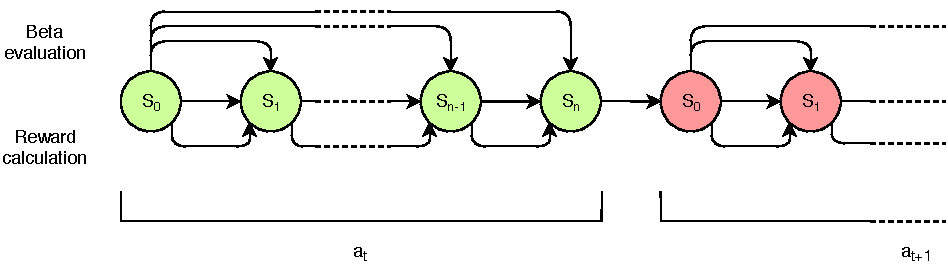
\includegraphics[width=120mm]{stateevolution.pdf}
	\caption{State evolution}
\end{figure}

Lastly, a finite length action history is tracked for the purposes of assigning negative rewards to deaths. When the agent dies, all actions in the action history are penalized, as the agent could have taken an action in this time frame that may have prevented its death but ultimately chose not to.An example of this is the agent being slightly off the edge of the stage and not choosing to jump back on. The action selected instead of jumping back on is then penalized.

